%====================================================================================================
\chapter{Introduction} \label{ch:introduction}
%====================================================================================================
The Standard Model of particle physics (\SM) is a remarkably successful theoretical framework that describes the known fundamental particles and their interactions via the electromagnetic, weak, and strong forces. It has been continuously validated through decades of experimental results and provides precise predictions that match observations.

However, the SM is not a complete theory of nature. It does not incorporate gravity, nor does it provide an explanation for the existence of dark matter, the possible realization of Super Symmetry (\SUSY), or the origin of neutrino masses. These open questions motivate the search for new physics beyond the Standard Model.

To probe these fundamental questions, high-energy particle colliders are essential to explore phenomena at smaller distance scales and higher mass thresholds. The Large Hadron Collider (\LHC), located at CERN, is the world's most powerful particle accelerator and was designed to explore fundamental physics at unprecedented energy scales. The LHC hosts four major experiments—ATLAS, CMS, ALICE, and LHCb—each designed to investigate different aspects of high-energy physics.

After the crucial discovery of the Higgs boson in 2012 at LHC, confirming the mechanism of electroweak symmetry breaking, the LHC entered a new phase of precision measurements and searches for rare processes. To further exploit its discovery potential and enhance sensitivity to rare processes, the LHC is currently undergoing a comprehensive upgrade call Phase-II upgrade. This Phase-II upgrade will lead to the High-Luminosity LHC (\HL-LHC), which aims to increase the instantaneous luminosity by a factor of five to seven, allowing more collision events to be recorded and improving the precision of physics measurements.

The following sections provide an overview of the LHC, the ATLAS experiment, and the upcoming Phase-II upgrade for the High-Luminosity LHC, followed by the motivation of this research. All these form the foundation for the research presented in this thesis.
%====================================================================================================
\section{The Large Hadron Collider} \label{sec:LHC}
%====================================================================================================
The Large Hadron Collider (\LHC) is the world’s most powerful particle accelerator, located 100~m underground at the European Organization for Nuclear Research (\CERN) near Geneva, Switzerland. It has a 27-kilometer circular tunnel, straddling the border between Switzerland and France. The LHC was designed to explore the frontiers of high-energy physics by colliding protons (and occasionally heavy ions such as lead nuclui) at unprecedented center-of-mass energies, providing unique opportunities to test the predictions of the Standard Model (SM) and to search for phenomena beyond it.

Protons are first accelerated using a series of smaller accelerators—like the LINAC, Proton Synchrotron (PS), and Super Proton Synchrotron (SPS)—before being injected into the LHC ring, where they are further accelerated. The LHC can achieve a center-of-mass energy of up to 14~TeV in proton-proton collisions currently, and is capable of delivering instantaneous luminosity exceeding $10^{34}~\mathrm{cm}^{-2}\mathrm{s}^{-1}$. Figure~\ref{fig:LHC_complex} provides an overall view of the LHC complex, including the main accelerator ring and the injector chain responsible for preparing and accelerating the particles prior to collision.

\begin{figure}[htbp]
  \centering
  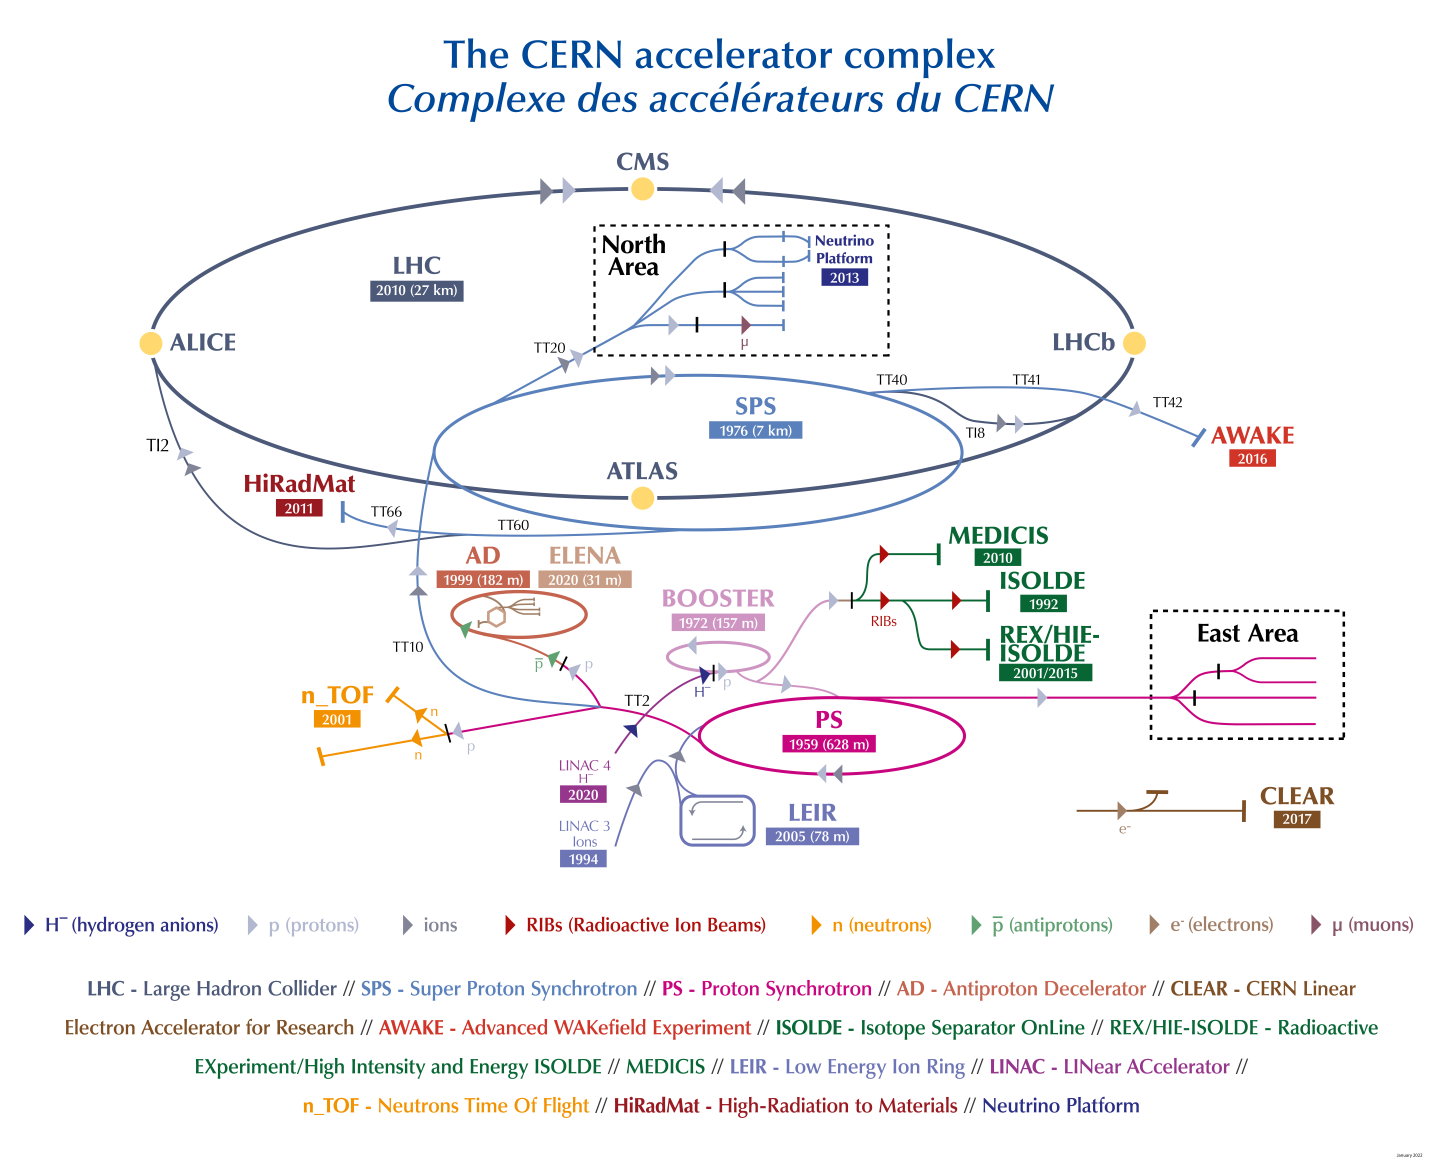
\includegraphics[width=1.0\textwidth]{figs/chapter1/LHC_complex.png}
  \caption{Overview of the LHC accelerator complex \cite{LHCComplex}.}
  \label{fig:LHC_complex}
\end{figure}

The LHC hosts four major experiments: ATLAS and CMS, which are general-purpose detectors designed to study a wide range of phenomena including Higgs boson production, Supersymmetry, and other physics beyond the SM; ALICE, which specializes in the study of the quark-gluon plasma in heavy-ion collisions; and LHCb, which specializes in rare decays of the $b$-quark sector.

One of the most significant achievements of the LHC to date is the discovery of the Higgs boson in 2012 by the ATLAS and CMS collaborations. This long-sought particle completes the Standard Model by confirming the mechanism of electroweak symmetry breaking through the Higgs field, which endows all elementary particles with mass. The observation of the Higgs boson not only validated a central component of the SM but also opened a new avenue for precision studies of the scalar sector and potential physics beyond the Standard Model.
%====================================================================================================
\section{The LHC-ATLAS Experiment} \label{ATLAS}
%====================================================================================================
The ATLAS (A Toroidal LHC ApparatuS) experiment is a general-purpose particle detector experiment located at one of the four main interaction points of the LHC, designed to explore physics phenomena from precise measurements of Standard Model parameters to the search for new particles and interactions. It is composed of several sub-detector systems arranged concentrically around the beam interaction point. Starting from the innermost region, the \textit{Inner Detector}, immersed in a solenoidal magnetic field, is designed to tracks charged particles and reconstructs their momenta, as well as precisely determining the position of vertices of the hardest scattering in interest. Surrounding the Inner Detector, the \textit{Calorimeter} system consists of electromagnetic and hadronic calorimeters, which measure the energy of electrons, photons, and hadrons through their interactions with dense absorber materials. The outermost layer is the \textit{Muon Spectrometer}, which detects muons that penetrate the inner layers, measuring their curvature in large toroidal magnetic fields to determine their momenta. The solenoidal magnetic field in the inner region, combined with the toroidal magnetic fields in the outer region, forms the \textit{Magnet System} and allows for precise momentum measurements over a wide energy range. A two-level trigger system is used to select events. In current LHC Run3 phase, the first-level trigger is implemented in hardware and uses a subset of the detector information to accept events at a rate below 100 kHz, which is followed by a software-based trigger that reduces the accepted event rate to 1 kHz. Also, a software suite framework named \textit{Athena} is widely used in data simulation process of the experiment.
A cut-away view of the ATLAS detector is shown in Figure~\ref{fig:ATLASDetector}.
\begin{figure}[htbp]
  \centering
  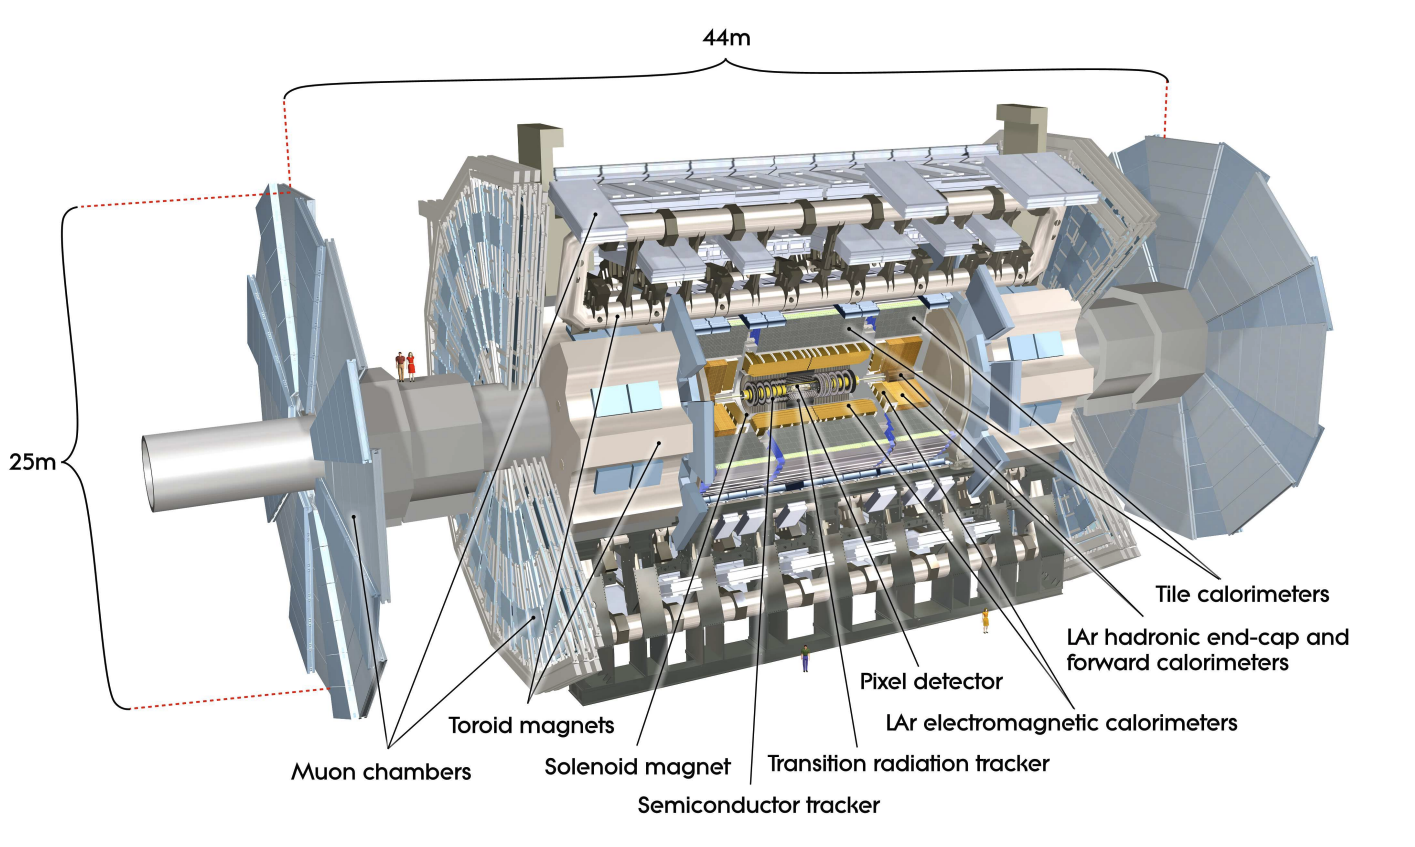
\includegraphics[width=1.0\textwidth]{figs/chapter1/ATLAS.png}
  \caption{Cut-away view of the ATLAS detector \cite{ATLASDetector2008}.}
  \label{fig:ATLASDetector}
\end{figure}
%====================================================================================================
\section{Phase-II Upgrade for HL-LHC} \label{sec:upgrade}
%====================================================================================================
As is pointed out at the begining of this chapter, to significantly enhance the sensitivity to rare processes and potential signatures beyond the SM, a thorough upgrade program is curretly underway: the Phase-II upgrade, which will lead to the High-Luminosity LHC (HL-LHC). As shown in Fig.~\ref{fig:HL-LHC}, the upgrade for HL-LHC is scheduled to start around 2026 and aims to dramatically increase the amount of data collection for physics analysis.

\begin{figure}[htbp]
  \centering
  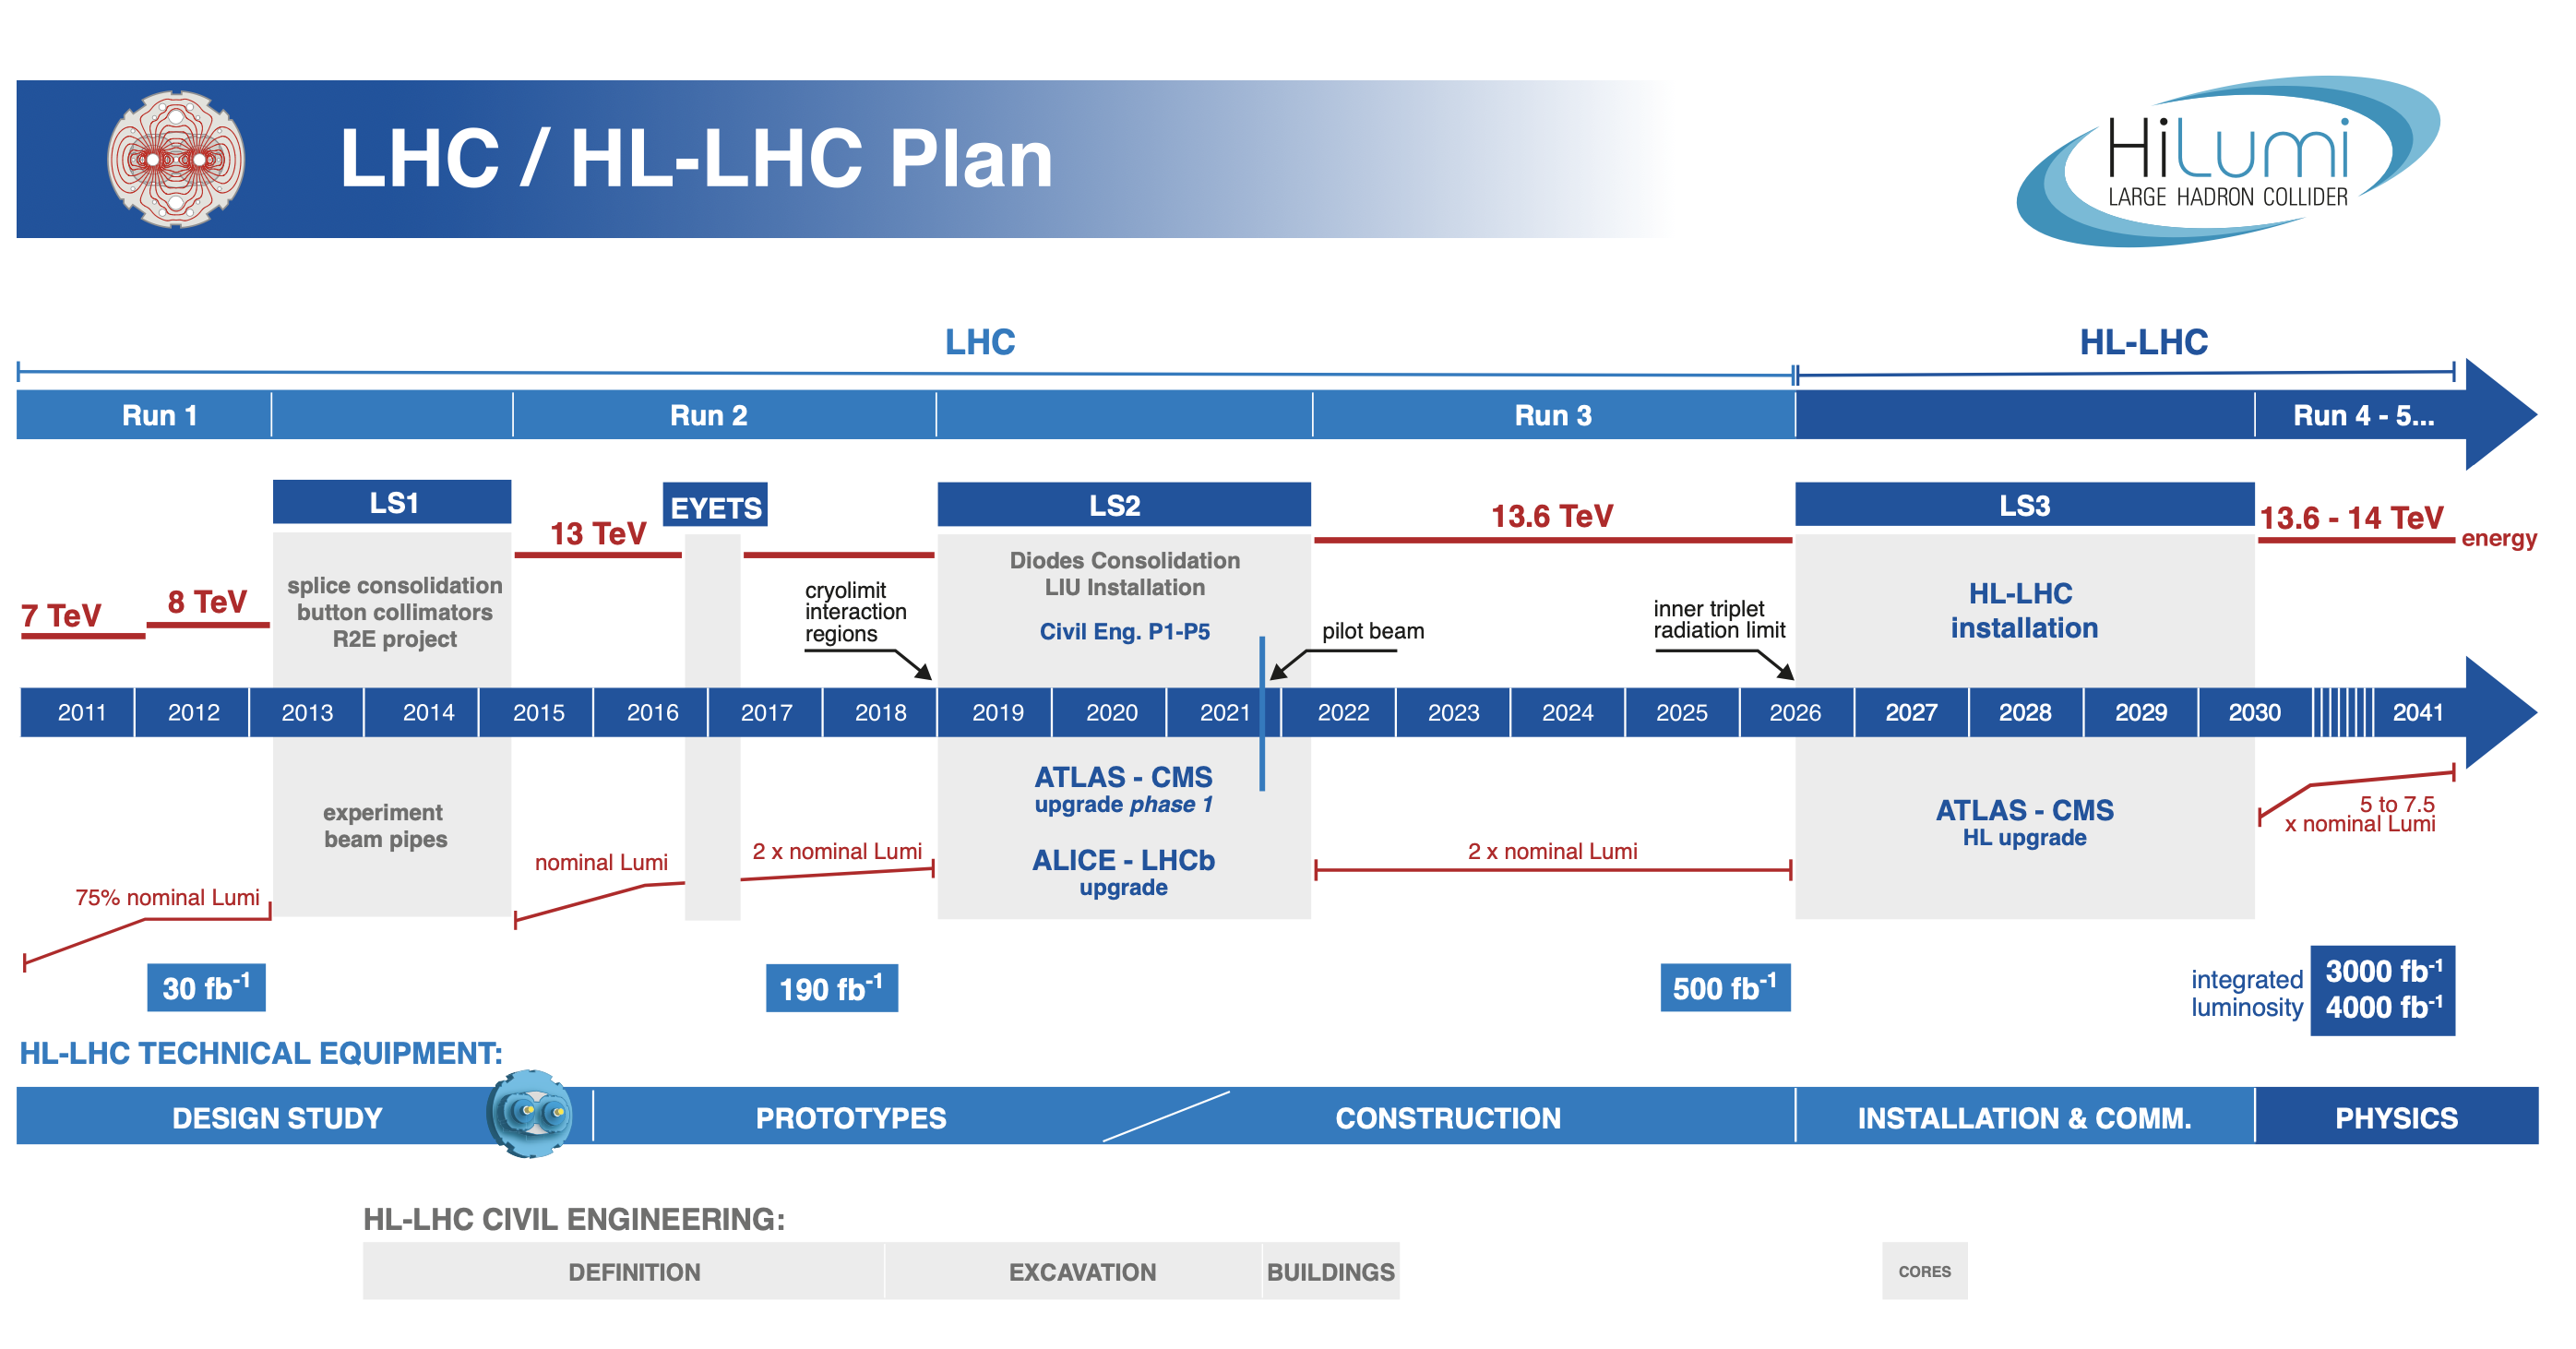
\includegraphics[width=1.0\textwidth]{figs/chapter1/HL-LHC_plan.pdf}
  \caption{HL-LHC schedule (last update January 2025) \cite{HL-LHC}.}
  \label{fig:HL-LHC}
\end{figure}

The HL-LHC will boost the instantaneous luminosity from the current $\sim 2 \times 10^{34}~\mathrm{cm}^{-2}\mathrm{s}^{-1}$ to a peak of $5$–$7.5 \times 10^{34}~\mathrm{cm}^{-2}\mathrm{s}^{-1}$ by increasing the number of protons per bunch and further focusing the beam at the collision points. Over a projected 10-year data-taking period, the HL-LHC is expected to deliver an integrated luminosity of up to $3,000~\mathrm{fb}^{-1}$. This increase in luminosity will result in a much higher number of simultaneous proton-proton interactions per bunch crossing, known as \textit{pile-up}, rising from an average of 50–65 in Run~3 to potentially 150–200 during HL-LHC operations (Run~4).

Such a large number of pile-ups poses a challenge to detectors in event reconstruction and background suppression processes. To meet these demands, the ATLAS detector will also undergo a upgrade to nearly all its major subsystems (sub-detectors). These include enhancements to the inner detectors, calorimeters, muon system, and particularly to the trigger and data acquisition (\TDAQ) system, which will be discussed in detail in Chapter~\ref{ch:ATLASforHLLHC}.

%====================================================================================================
\section{Motivation and Structure of this Thesis} \label{sec:motivation}
%====================================================================================================
This thesis focuses on the development of a software simulation framework for the upgraded muon trigger system in the ATLAS experiment for the HL-LHC. In the HL-LHC phase, the instantaneous luminosity will significantly increase, resulting in a much higher number of events per bunch crossing. To meet the requirements, the ATLAS muon trigger system will undergo a complete upgrade. As a part of that, the Thin Gap Chamber (\TGC), at the endcap region of the muon trigger system, will have the digital electronics and firmware logic entirely replaced and upgraded. In order to validate and support the development of the new firmware, a corresponding software simulation is necessary. 

As a preliminary step, this study first performs an update and evaluation of the existing simple emulator for L0 muon trigger system, to assess the current trigger performance, including both barrel and endcap regions. This analysis confirms, as a result, the necessity for a precise and detailed simulator that emulates real trigger logic. Then, as a concrete example, as well as the core of this research, the development of simulation of the endcap TGC Sector Logic (\SL) was performed on the base of an existing bitwise simulator. In this part, a bitwise-level simulator was developed and integrated into the ATLAS software framework, Athena, ensuring consistent logic behavior. To satisfy Athena’s memory constraints, a strategy for optimizing the storage of Look-Up Table (LUT) was also devised and applied. Finally, Monte Carlo simulation samples were used as input to validate the implementation and evaluate its trigger performance.

This thesis is structured as follows: Chapter~\ref{ch:ATLASforHLLHC} provides an overview of the LHC-ATLAS experiment, along with the upgrade for the HL-LHC. Chapter~\ref{ch:ATLASSoftwareFramework} introduces the ATLAS software framework, Athena. Chapter~\ref{ch:L0MuonEmulator} presents the update to an emulator for L0 muon trigger system, followed by an assessment of its limited performance. Chapter~\ref{ch:L0MuonS1TGC} describes the implementation and optimization of the simulator for TGC SL. Chapter~\ref{ch:PerformanceEvaluation} presents the Monte Carlo simulation setup and performance evaluation.